\section{Results}

\subsection{Estimating traits via PROSPECT inversion}

\begin{figure}
  \includegraphics{{figures/prospect_pairs.N}.pdf}
  \caption{Inter-version comparison of estimates of number of leaf mesophyll layers.}
  \label{fig:prospect_pairs_N}
\end{figure}

\begin{figure}
  \includegraphics{{figures/prospect_pairs.Cab}.pdf}
  \caption{Inter-version comparison of estimates of number of total leaf chlorophyll content.}
  \label{fig:prospect_pairs_Cab}
\end{figure}

\begin{figure}
  \includegraphics{{figures/prospect_pairs.Car}.pdf}
  \caption{Inter-version comparison of estimates of number of total leaf carotenoid content.}
  \label{fig:prospect_pairs_Car}
\end{figure}

\begin{figure}
  \includegraphics{{figures/prospect_pairs.Cw}.pdf}
  \caption{Inter-version comparison of estimates of number of total leaf water content.}
  \label{fig:prospect_pairs_Cw}
\end{figure}

\begin{figure}
  \includegraphics{{figures/prospect_pairs.Cm}.pdf}
  \caption{Inter-version comparison of estimates of number of total leaf dry matter content.}
  \label{fig:prospect_pairs_Cm}
\end{figure}

%TODO: Find a more concise way to represent these results

The extent of agreement on trait estimates between different versions of PROSPECT was strongly trait-dependent.
In general, traits that influence leaf reflectance over a broader range (number of mesophyll layers---Figure~\ref{fig:prospect_pairs_N}---,water content---Figure~\ref{fig:prospect_pairs_Cw}---,and dry matter content---Figure~\ref{fig:prospect_pairs_Cm}) agreed better than parameters that affected reflectance over specific, narrow spectral regions (concentrations of chlorophyll---Figure~\ref{fig:prospect_pairs_Cab}---and carotenoids---Figure~\ref{fig:prospect_pairs_Car}).
The most significant differences were in estimates of carotenoid concentrations between PROSPECT 5/5B and D (Figure~\ref{fig:prospect_pairs_Car}).

\begin{figure}
  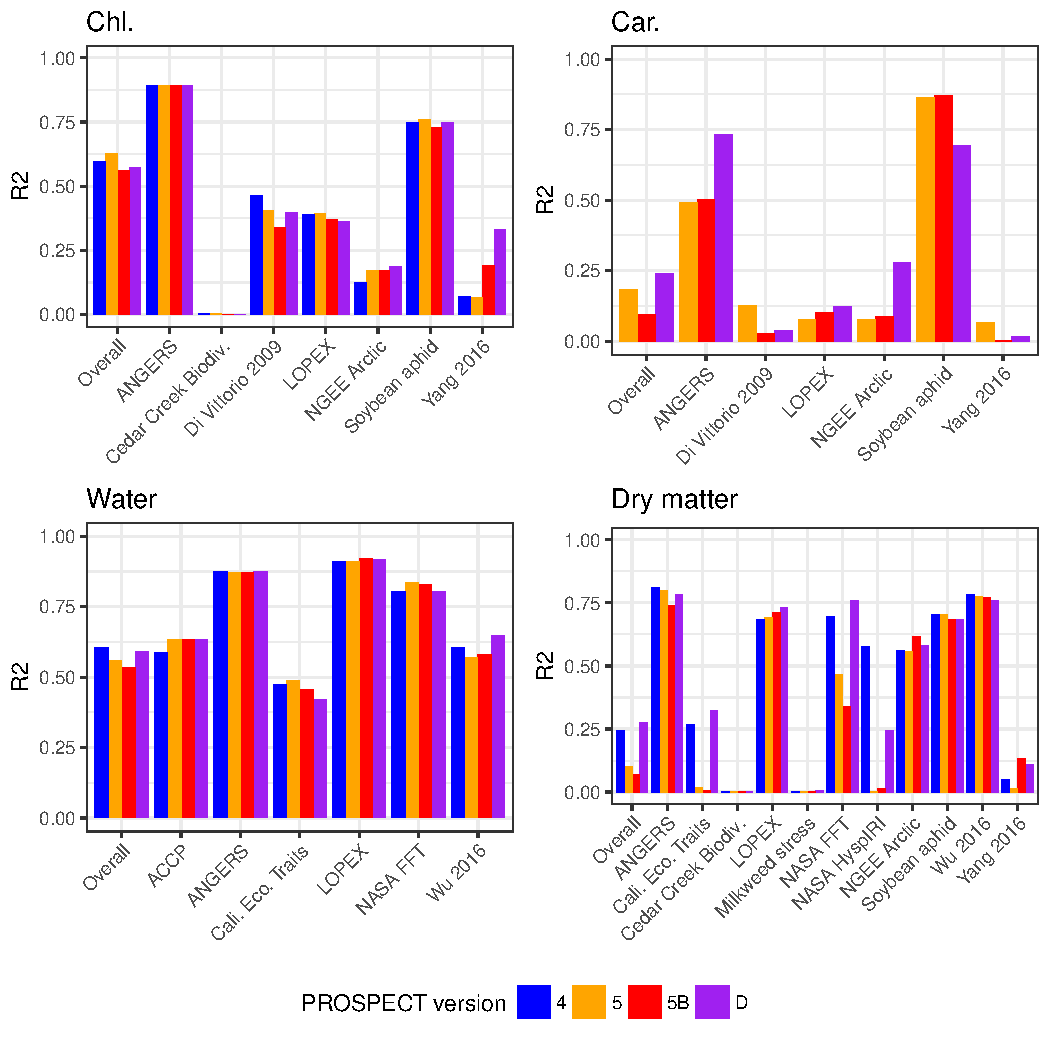
\includegraphics{{figures/project_validation_summary}.pdf}
  \caption{Validation of PROSPECT against observed trait values, by project and PROSPECT version}
  \label{fig:project_validation_summary}
\end{figure}

Across most projects and traits, the four different PROSPECT versions performed similarly in terms of their ability to retrieve traits (Figure~\ref{fig:project_validation_summary}).
For all versions of PROSPECT, leaf water content was consistently the most accurate trait retrieved, while retrievals of other traits were highly project-specific.
Inversion accuracy also varied significantly by project, which can largely be explained by differences in the species sampled across different projects (Supplementary Figures~\ref{fig:error_speciesbyproj_Cab}-\ref{fig:error_speciesbyproj_Cm}).
Because PROSPECT-D also retrieves anthocyanin content and generally performed as well or better than other versions, it was the version selected for subsequent analyses.
A more detailed validation for PROSPECT-D is shown in Figure~\ref{fig:prospect_D_validation}.

%TODO: More here?

\begin{figure}
  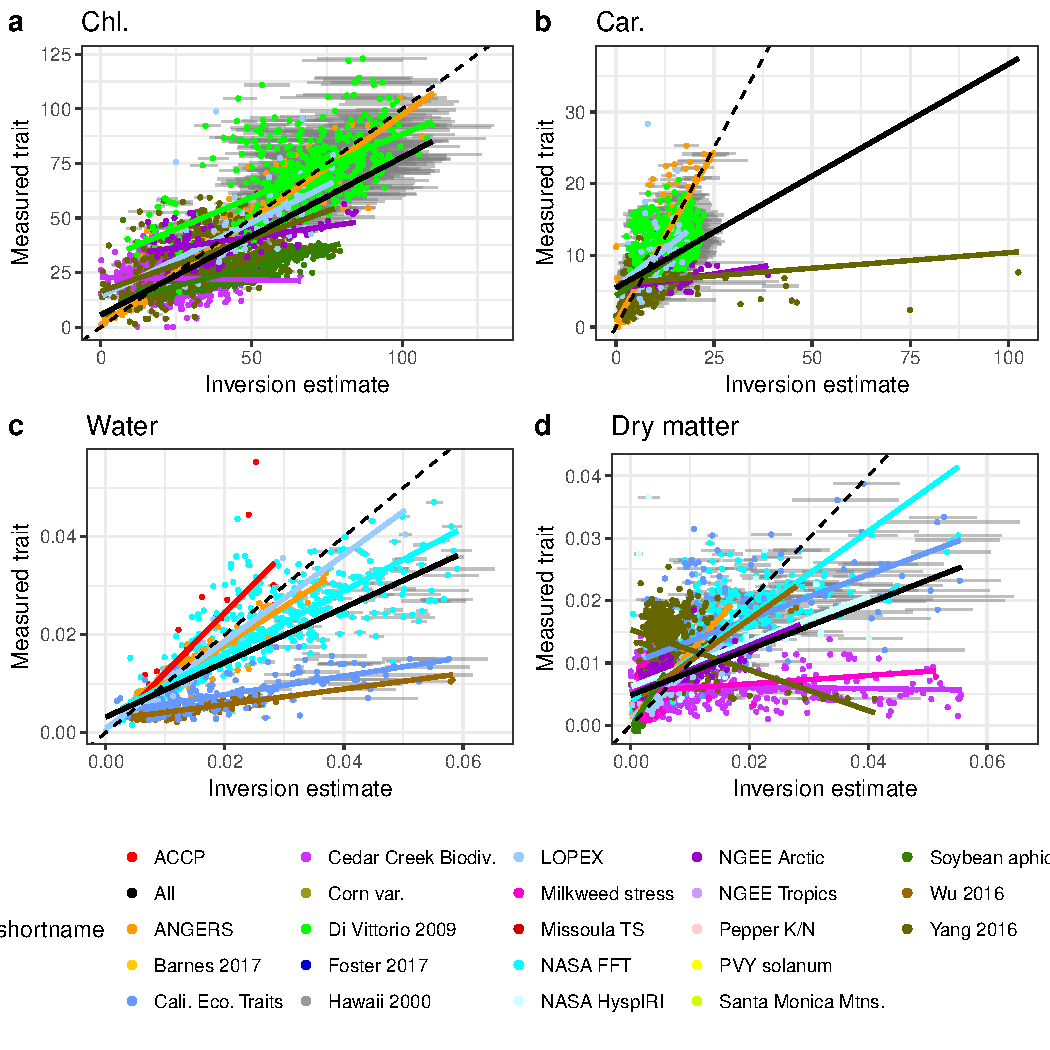
\includegraphics{{figures/prospect_D_validation}.pdf}
  \caption{\
  Validation of PROSPECT-D against observed trait values.
  Grey lines indicate 95\% confidence intervals around trait estimates.
  Solid, colored lines are least-squares regressions fit to the data by project.
  The solid black line is a regression fit to all of the data all at once.
  The dashed black line is a 1 to 1 fit.
}
  \label{fig:prospect_D_validation}
\end{figure}

\subsection{Intraspecific variability in leaf traits}


